\chapter{Implementación del flujo de trabajo}
\label{ch:especifico2}

Como se pudo observar en el capítulo \ref{ch:especifico1}, se realizó la selección de la tarjeta de desarrollo Zedboard para el desarrollo del proyecto, además de esto uno de los parámetros que se tomó en cuenta fue la compatibilidad de esta tarjeta con el flujo de trabajo de Yocto Project, es por esto que en este capítulo se pretenden establecer los flujos de trabajo para el prototipado de algoritmos de control de orientación y navegación para aplicaciones espaciales. Esto mediante el uso de MATLAB Simulink para tomar un caso de uso como ejemplo, seguido de esto convertir el código por medio de la transformación de modelo de Simulink a un modelo de código C, esto con el objetivo de poder embeber el código C en una imagen mínima por medio del flujo de trabajo de Yocto Project y finalmente probar el mismo en la tarjeta de desarrollo seleccionada en el capítulo \ref{ch:especifico1} y de esta forma poder comparar los resultados obtenidos y el tiempo de ejecución que llevo la tarea en el computador y en el sistema embebido.


\begin{figure}[h!]
    \centering
    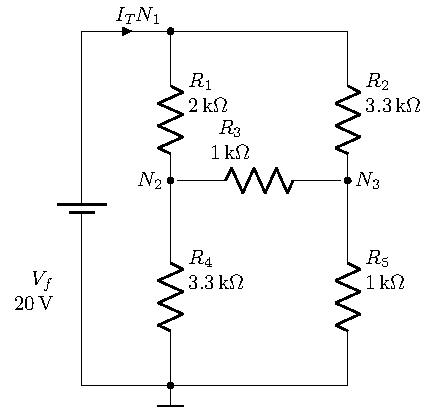
\includegraphics[width=0.5\textwidth]{fig/figtemplate.pdf}
    \caption{Diagrama general del flujo de trabajo propuesto}
    \label{fig:diagrama_flujo_trabajo}
\end{figure}


En la Figura \ref{fig:diagrama_flujo_trabajo}, se muestra un diagrama del flujo de trabajo general. En este capítulo se trabajará en la sección remarcada en rojo la cual engloba la generación del modelo utilizado como caso de uso, la validación del mismo en MATLAB Simulink, la generación de un código en lenguaje C y la incorporación del mismo en el flujo de trabajo de Yocto Project.


\section{GNC embebido software workflow}

Anteriormente definimos un flujo de trabajo para poder establecer el prototipado de algoritmos de control, orientacion y navegacion para aplicaciones espaciales, el mismo prentendemos logaralo mediante la seleccion de un caso de estudio en matlab simulink el cual se mostrara en el desarrollo de este capitulo

\section{Flujo de trabajo de la aplicación Model 2 Model Transformation}
caso de estudio matlab embedded coder


\subsection{Seleccion del caso de estudio}

se selecciona cualquier aplicacion de simulink con el fin de lograr demostrar el funcionamiento del sistema

\subsection{Simulacion del caso de estudio en Matlab Simulink}

se simula el caso seleccionado para su ejecucion 

\subsection{Resultados obtenidos con la ejecucion de la simulacionn}

se presentan los reusltados obtenidos ejecutando la simulacion en el computador host

\subsection{Simulink coder}

inicio del flujo de simulink coder 

\subsubsection{Definicio de paramtetros}

definicion de los parametros basicos de operacion

\subsubsection{seleccion del procesador objetivo}

se selecciona el procesador y la arquitectura del mismo

\subsubsection{Seleccion del tipo de archivo de construccion}

Se selecciona cmake como archivo de compilacion 

\subsubsection{Generacion de archivos de compilacion}

se le da build a la imagen de ejecucion

\subsection{Contenedor para compilacion de los binarios}

se geenra un container por emdio de docker io, este debera de ejecutar la imafen dew linux 20.04 esto debido a la dependencia de la libreria GCC 2.30 que presenta yocto a la hora de compilar los arhcivoso
se instalan las herramientas requeridas

\subsubsection{Istalacion de programas en el contenedor}

instalamos el cross compiler y las dependencias del mismo

\subsection{Compilacion de los binarios}

Compilamos los binarios para su ejecucion en

Una vez compilados los binarios se puede continuar con el flujo que se presneta en el diagrama que se muestra en la Figura XX, lo cual seria la implemetnacion de los binarios en una imagen de yocto. mediante los pasos que se muestran en la siguiente seleccion


\subsection{Caso de estudio}


\section{Flijo de Trabajo Herramienta desarrollada por mi persona}
Diagrama de pasos para poder ejecutar el flujo de trabajo

\subsection{Sistema operativo para desarrollo}
hablar sobre el sistema operativo base que se reqiere para generar el flujo, version de kernel y demas daros 

\subsection{Generacion de un contenedor}
por que se debe de utilizar un contenedor para fines del proyecto
\subsubsection{Creacion de un usuario no root}
por que se requiere generar un usuario no root 
\subsection{Yocto Project}
referencar al marco teorico de que es y para que se esta utilizando en el desarrollo del marco de trabajo
\subsection{creacion de una capa de yocto}
como se debe de generar una capa en yocto
\subsection{Caso de estudio}
\subsection{integracion del programa generado a la capa de yocto}
como se debe de intgrar y para que funciona cada comando del .bb de la capa
\subsection{Generacion de la imagen minima}
Por que se usa una imagen minima 
\subsection{Implementacion de la imagen minima en la tarjeta de desarrollo zedboard}
Como se debe de implementar el boot de la tarjeta, como se debe de implementar el  sistema de archivos
\subsection{Conexion de la tarjeta de desarrollo con el computador host}
diagrama de conexion y programas utilizados para llevar a cabo el enlace

\subsection{Ejecucion del caso de estudio y resultados}

\subsection{Comparacion de resultados}

\section{Reflexion final}